\subsection{The Halved Model}

The idea behind the halved model is that the model we have can be looked at in a different way than it was introduced in.
We know the model maps an input $x$ to $f(x) \mod 1$, meaning that if the output $f(x)$ is greater or equal to 1, we subtract 1 from it until it is in the range $[0, 1)$.
Similarly, we add 1 to it if it is smaller than 0 until it is in the desired range.
Now instead of confining the model to the domain of $[0, 1)$, we think of it repeating infinitely in both directions.
We can achieve this by mapping $x$ to $f(x - \lfloor x \rfloor)$.
This trick maps the input $x$ into the domain, on which our model function produces sensible results and causes it to repeat infinitely.
\Cref{fig:minrep.infinite.model.concept} illustrates this concept for the cycle $P_7^3$.
The blue square is the full model.
One can see, that the branch $f_\D$ is outside the blue square at its right edge.
This is because it was cut off and continued at the bottom of the square before, due to the $\mod 1$ operation.

\todo{this makes sense in the original problem domain}

In this model, there are no cycles that have multiple rotations.
Instead, the cycles that had multiple rotations in the full model, manifest as a sequence of different blocks of the full model.
Meaning for the example $P_7^3$, the same blocks of $\A^4\B^3\C^4\D^3$ are repeating infinitely.
But for an example with multiple rotations, such as $\A\B\C\D\A^2\B^2\C^2\D^2$, the blocks will not all be the same.
Instead, the blocks $\A\B\C\D$ and $\A^2\B^2\C^2\D^2$ will be alternating.

Now the symmetry of our function $f$ comes into play.
Since $f(x + 0.5) = f(x) + 0.5$ for $x \in [0, 0.5)$, we can split the infinite model into smaller blocks than the blue block of the full model.
The function of the infinite model repeats in blocks of size 0.5, these blocks are marked red in \Cref{fig:minrep.infinite.model.concept}.
These red blocks represent the halved model, it is the smallest repeating part of the infinite model.
To get the cycle in the halved model, we look at the pattern in which different red blocks repeat along the infinite model.
For our example in the picture, there is only one red block that repeats infinitely, $\L^4\R^3$.
The next section will explain, how to translate cycles between the halved and full model.

\begin{figure}
	\centering
	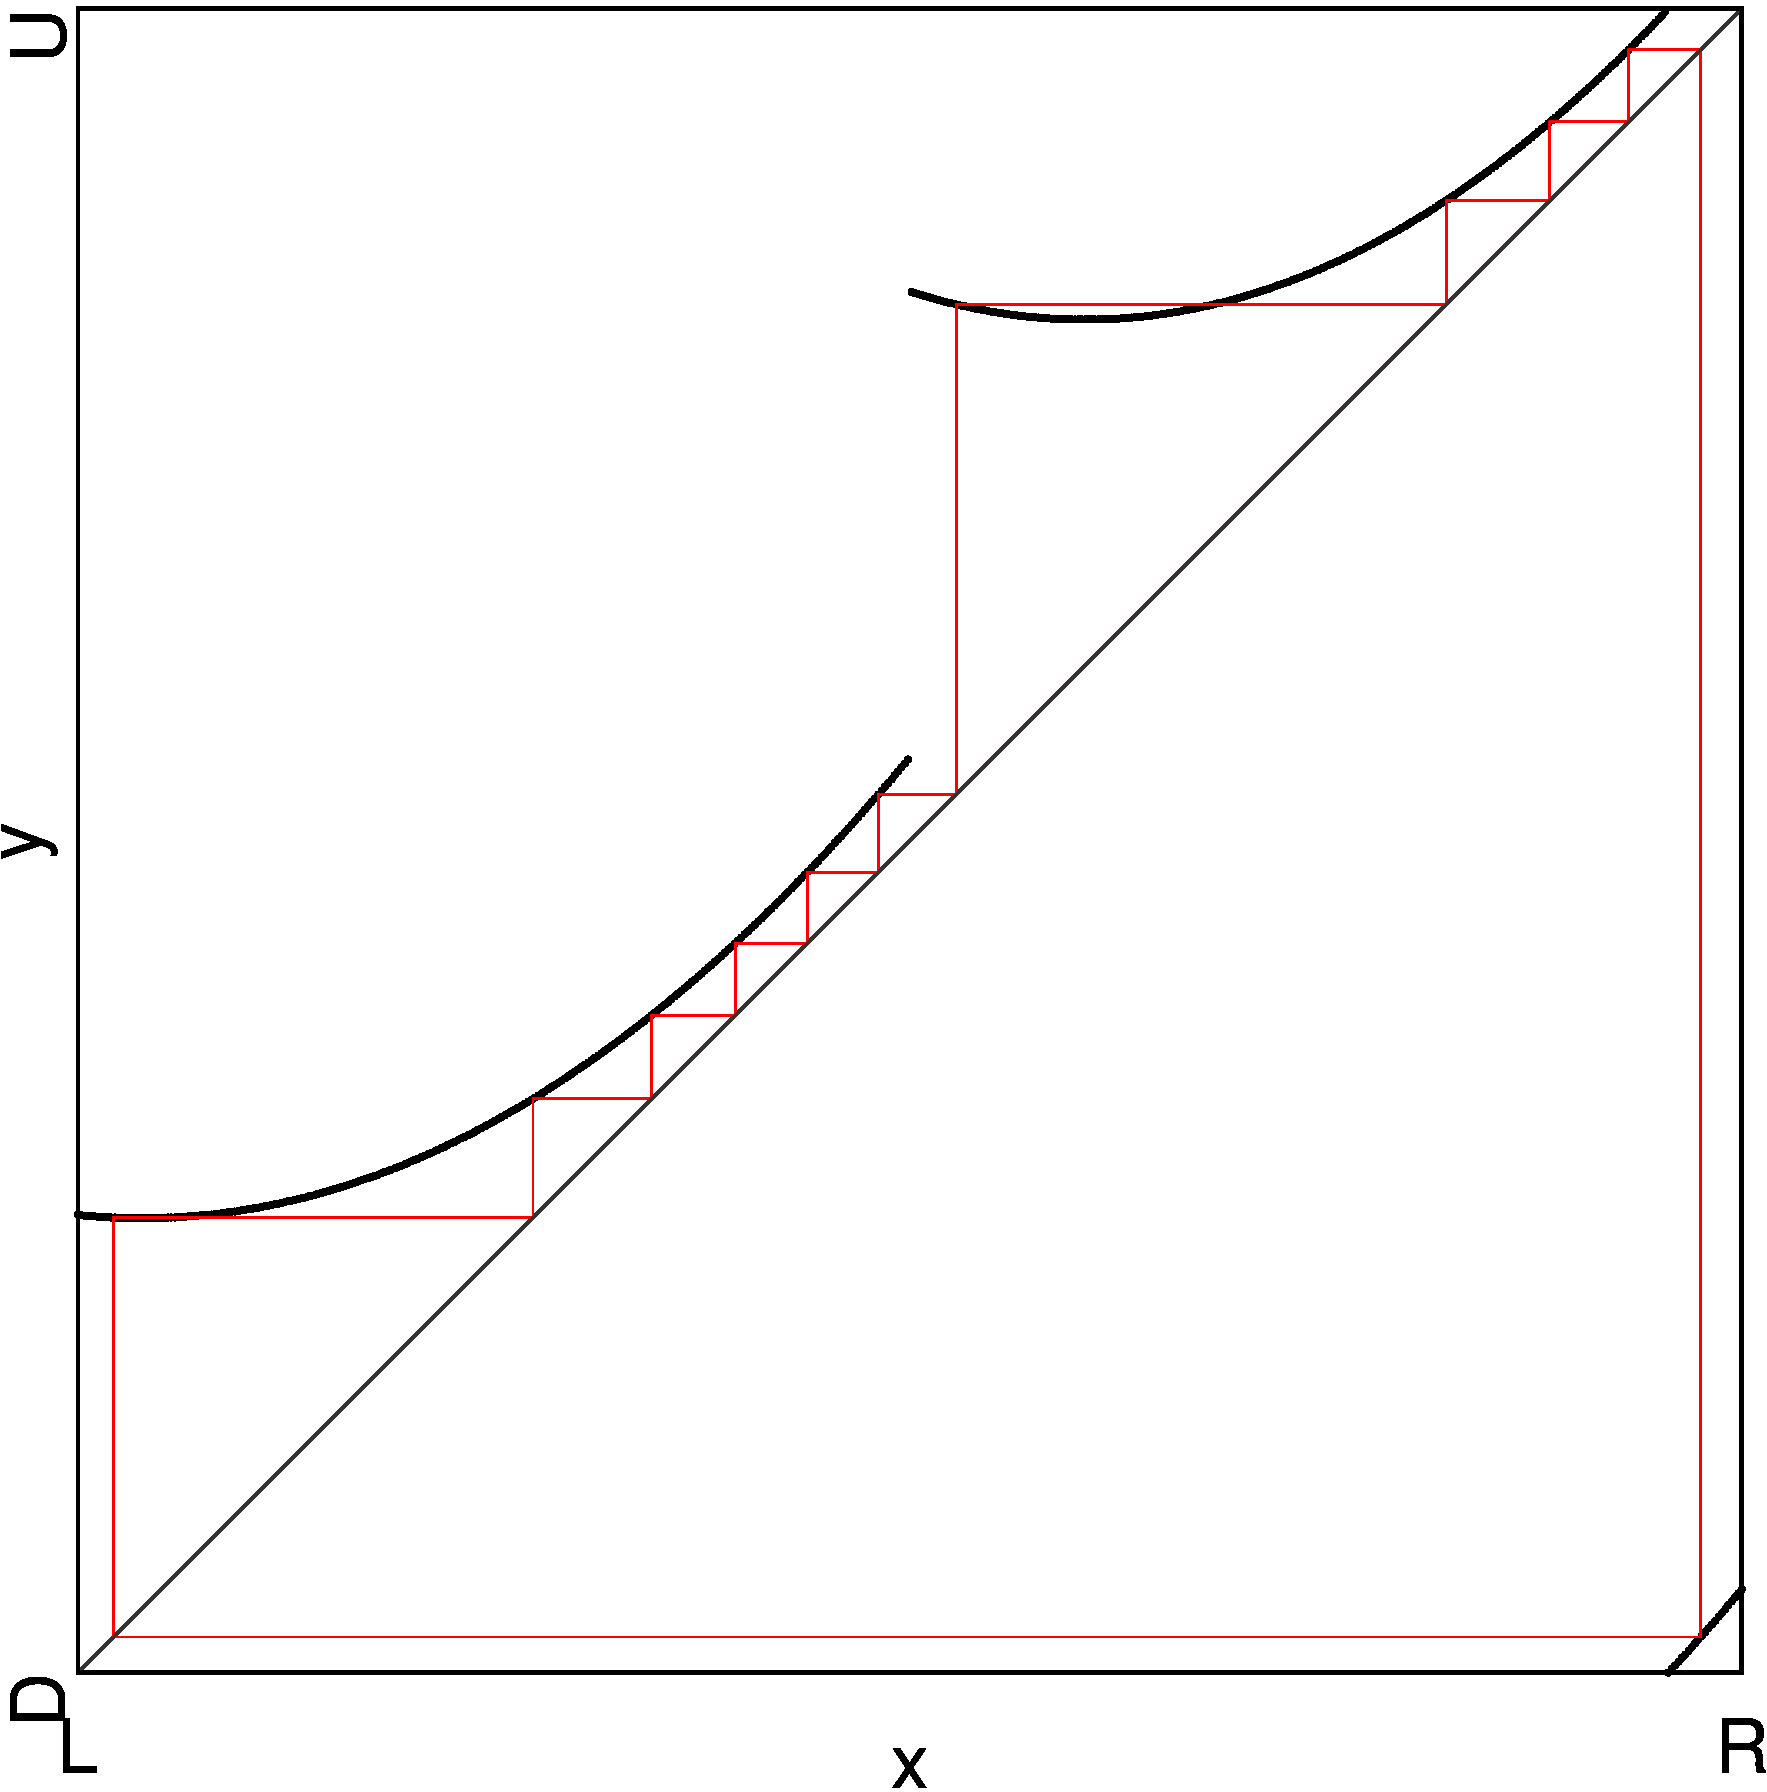
\includegraphics[width=.7 \textwidth]{63_MinimalRepr_Adding_Halved/Cob_Vis_s/Manual/result.png}
	\caption{Illustration of the infinite model concept.}
	\label{fig:minrep.infinite.model.concept}
\end{figure}

\subsubsection{Naive Algorithm}

Based on this concept of the infinite model, one can formulate a naive algorithm for translating symbolic sequences between the halved and full model.
We will start with the easier direction from the full to the halved model.
From this direction we can't learn much about the nature of the period-adding structure in the full model, the inverse will be more important for that.

To translate a symbolic sequence of the full model we start by writing it down.
For example $\A^4\B^3\C^4\D^3$.
Then we replace the symbols $\A$ and $\C$ by $\L$ and the symbols $\B$ and $\D$ by $\R$.
Now we have $\L^4\R^3\L^4\R^3$.
Finally, we have to check for redundancy in the resulting cycle.
In our example, the cycle $\L^4\R^3$ repeats twice in $\L^4\R^3\L^4\R^3$, so we just keep $\L^4\R^3$.
\todo{explain using the illustration}

The inverse is trickier.
We start by writing down the symbolic sequence in the halved model.
For example $h = \L^4\R^3\L4\R^3\L^3\R^3$.
Now we need to build pairs of rotations since each blue block fits two red blocks.
If there is one rotation left over at the end, we wrap around or equivalently write down the original sequence again.
We repeat this until we fit all rotations that we have written down.

\begin{lemma}
	\label{lemma:writing.down}
	For cycles in the halved model $h$ with an even number of rotations $n$, we only need to write the original cycle down once.
	For cycles in the halved model $h$ with an odd number of rotations $n$, we need to write the original cycle down exactly twice.
\end{lemma}

\begin{proof}
	\begin{enumerate}
		\item Let $n = 2i$. Then, we can build $i$ pairs of rotations and fit all $2i$ rotations of the original model.
		\item Let $n = 2i + 1$. We start by building $i$ pairs of rotations, fitting $2i$ rotations.
		      This will leave the last rotation unpaired o we write down the sequence of $2i + 1$ rotations again.
		      Now we can pair up the last rotation of the first sequence we wrote down with the first rotation of the sequence we just wrote down.
		      $2i$ rotations remain, which we can fit into $i$ pairs.
	\end{enumerate}
\end{proof}

Notice, our example symbolic sequence has 3 rotations.
This means we have to write down the original sequence twice $h^2 = \L^4\R^3\L4\R^3\L^3\R^3\L^4\R^3\L4\R^3\L^3\R^3$.

Then we pair up the rotations, this corresponds to drawing blue boxes around the red boxes in the infinite model.
In our example, we get the pairs $(\L^4\R^3\L^4\R^3)(\L^3\R^3\L^4\R^3)(\L^4\R^3\L^3\R^3)$.
The pairs then have to be translated using the function $t$ defined below.
The resulting symbolic sequence is $T(h) = \A^4\B^3\C^4\D^3\A^3\B^3\C^4\D^3\A^4\B^3\C^3\D^3$.

\begin{definition}
	The function $t$ maps two rotations of a symbolic sequence in the halved model to a single rotation in the full model.
	It is defined in the following way.
	\begin{align}
		t: & \L^a\R^b\L^c\R^d \mapsto \A^a\B^b\C^c\D^d
	\end{align}
\end{definition}

\begin{definition}
	The function $s$ shifts a symbolic sequence in the halved model by a single rotation.
	Let $\tau_1\tau_2 \dots \tau_n$ be a sequence in the halved model, where each $\tau_i$ is one rotation.
	Then $s$ is defined in the following way.
	\begin{align}
		s: & \tau_1\tau_2 \dots \tau_n \mapsto \tau_2 \dots \tau_n\tau_1
	\end{align}
	In the full model, there is a similar function, $s'$, that shifts a symbolic sequence in the full model by a single rotation.
	Let $\tau'_1\tau'_2 \dots \tau'_n$ be a sequence in the full model, where each $\tau'_i$ is one rotation.
	The $s'$ is defined in the following way.
	\begin{align}
		s': & \tau'_1\tau'_2 \dots \tau'_n \mapsto \tau'_2 \dots \tau'_n\tau'_1
	\end{align}
\end{definition}

\begin{definition}
	The two symbolic sequences $\sigma$ and $\rho$ in the full model are shift-equivalent $\sigma \equiv \rho$,
	if they both have the same number of rotations $n$
	and there is a number $0 \leq i < n$, such that $\sigma = s'^i(\rho)$.
	Where $s'^i$ is the same as applying $s'$ $i$ times.
\end{definition}

We need to repeat the whole process for each shift $s^i$ of the original symbolic sequence for $0 < i < n$ where $n$ is the number of rotations of the original symbolic sequence.
And we only keep the results that are not shift-equivalent to any previous result.
In our example, we would repeat the process for $s(h) = \L^4\R^3\L3\R^3\L^4\R^3$ and get the result $T(s(h)) = \A^4\B^3\C^3\D^3\A^4\B^3\C^4\D^3\A^3\B^3\C^4\D^3$.
This result is shift-equivalent to the first result by shifting it 2 times.
Last we need to repeat it for $s^2(h) = \L^3\R^3\L4\R^3\L^4\R^3$ and get the result $T(s^2(h)) = \A^3\B^3\C^4\D^3\A^4\B^3\C^3\D^3\A^4\B^3\C^4\D^3$.
This result is shift-equivalent to the first result by rotating it once.

Therefore the cycle $h$ in the halved model manifests as a single cycle $T(h)$ in the full model.
We write it as $F(h) = \{T(h)\} = \{\A^4\B^3\C^4\D^3\A^3\B^3\C^4\D^3\A^4\B^3\C^3\D^3\}$.
The result of $F$ is a set because the cycle $h$ in the halved model may manifest as multiple coexisting cycles in the full model.

\subsubsection{Insights}
\todo{better heading}

With this naive algorithm, we can start to investigate rules for the period-adding structure in the full model.

\begin{lemma}
	\label{lemma:equivalence.translations}
	The translations of the two cycles $h_1$ and $h_2 = r^{2i}(h_1)$ in the halved model are shift-equivalent $T(h_1) \equiv T(h_2)$ for all integers $i$.
\end{lemma}

\begin{proof}
	Let $h_1 = \tau_1\tau_2 \dots \tau_n$, therefore $h_2 = \tau_{2i+1} \dots \tau_n\tau_1 \dots \tau_{2i}$.
	The translations are $T(h_1) = t(\tau_1\tau_2)t(\tau_3\tau_4) \dots t(\tau_{n-1}\tau_n)$
	and $T(h_2) = t(\tau_{2i+1}\tau_{2i+2}) \dots t(\tau_{n-1}\tau_n)t(\tau_1\tau_2) \dots t(\tau_{2i-i}\tau_{2i})$.
	We can see that $T(h_2) = s'^i(T(h_1))$ and therefore $T(h_1) \equiv T(h_2)$.
\end{proof}

\begin{theorem}
	\label{theorem:coexistence.even}
	The mainfestations of a cycle in the halfed model $h$ is either $F(h) = \{T(h), T(s(h))\}$ or $F(h) = \{T(h)\}$.
	And \begin{enumerate}
		\item $F(h) = \{T(h), T(s(h))\}$ if the number of rotations of the sequence $h$ is even.
		\item $F(h) = \{T(h)\}$ if the number of rotations of the sequence $h$ is odd.
	\end{enumerate}
\end{theorem}

\begin{proof}
	Let $h = \tau_1\tau_2 \dots \tau_n$ a symbolic sequence in the halved model with $n$ rotations.
	We know from \Cref{lemma:equivalence.translations} that the only possible candidates for $F(h)$ are $T(h)$ and $T(s(h))$.
	These are the first two possibilities we check in the algorithm and all other shifts $T(s^i(h))$ with $2 \leq i < n$ are shift-equivalent to $T(h)$ or $T(s(h))$.
	So, in the following, we will only check for the shift-equivalence of these two candidates.
	\begin{enumerate}
		\item Let $n = 2i$.
		      From \Cref{lemma:writing.down} we know that we only need to write down the original cycle $h$ once and thus we get the following translations.
		      \begin{align*}
			              & T(h) = t(\tau_1\tau_2) t(\tau_3\tau_4) \dots t(\tau_{n-1}\tau_n) \\
			      \nequiv & T(h) = t(\tau_2\tau_3) t(\tau_4\tau_5) \dots t(\tau_n\tau_1)
		      \end{align*}
		      The two candidates are not shift-equivalent because the pair $t(\tau_1\tau_2)$ in $T(h)$ is not included in the other candidate $t(s(h))$.
		      The same is true for any other pair, and therefore $F(h) = \{T(h), T(s(h))\}$.
		\item Let $n = 2i + 1$.
		      From \Cref{lemma:writing.down} we know that we need to write down the original cycle $h$ exactly twice and thus we get the following translations.
		      \begin{align*}
			             & T(h) = t(\tau_1\tau_2) t(\tau_3\tau_4) \dots t(\tau_n\tau_1) t(\tau_2\tau_3) \dots t(\tau_{n-1}\tau_n) \\
			      \equiv & T(h) = t(\tau_2\tau_3) \dots t(\tau_{n-1}\tau_n) t(\tau_1\tau_2) t(\tau_3\tau_4) \dots t(\tau_n\tau_1)
		      \end{align*}
		      The two candidates are shift-equivalent.
		      By shifting the second candidate $T(s(h))$ $2i$ times, we get the first candidate $T(h)$.
		      Therefore, the second candidate is discarded and $F(h) = \{T(h)\}$.
	\end{enumerate}
\end{proof}

Note that a result of $F(h) = \{T(h), T(s(h))\}$ means that the cycle in the halved model $h$ manifests as two coexisting cycles in the full model.
With this knowledge, we now can explain, why some cycles in the full model have a much lower period than expected in period-adding structures.

\begin{lemma}
	\label{lemma:t.preserves.period}
	The function $t$ preserves the period. $|\tau_1\tau_2| = |t(\tau_1\tau_2)|$.
\end{lemma}

\begin{proof}
	Let $\tau_1\tau_2 = \L^a\R^b\L^c\R^d$.
	\begin{align*}
		|\tau_1\tau_2| =  |\L^a\R^b\L^c\R^d|
		= a + b + c + d
		= |\A^a\B^b\C^c\D^d|
		= |t(\L^a\R^b\L^c\R^d)|
		= |t(\tau_1\tau_2)|
	\end{align*}
\end{proof}

\begin{theorem}
	\begin{enumerate}
		\item If a cycle in the halved model manifests as two coexisting cycles in the full model, the period of either cycle is the same as the period of the cycle in the halved model. $|T(h)| = |T(r(h))| = |h|$.
		\item If a cycle in the halved model manifests as a single cycle in the full model, the period of this cycle is double the period of the cycle in the halved model. $|T(h)| = 2 |h|$.
	\end{enumerate}
\end{theorem}

\begin{proof}
	\begin{enumerate}
		\item From \Cref{theorem:coexistence.even} we know that if the cycle $h$ in the halved model manifests as two coexisting cycles in the full model, $h$ has an even number of rotations $n$.
		      And its translation is $T(h) = t(\tau_1\tau_2) t(\tau_3\tau_4) \dots t(\tau_{n-1}\tau_n)$.
		      Combining this with the fact, that $t$ preserves the period of its input as described in \Cref{lemma:t.preserves.period}, we can calculate the period of $T(h)$ in the following way.
		      \begin{align*}
			      |T(h)| & = |t(\tau_1\tau_2) t(\tau_3\tau_4) \dots t(\tau_{n-1}\tau_n)|           \\
			             & = |t(\tau_1\tau_2)| + |t(\tau_3\tau_4)| + \dots + |t(\tau_{n-1}\tau_n)| \\
			             & = |\tau_1\tau_2| + |\tau_3\tau_4| + \dots + |\tau_{n-1}\tau_n|          \\
			             & = |\tau_1\tau_2 \dots \tau_n| = |h|
		      \end{align*}
		      So the period of the cycle $T(h)$ in the full model is the same as the period of the cycle $h$ in the halved model.
		      The same calculation can be done for $T(s(h))$ and is omitted here.
		\item Similarly we know that if the cycle $h$ in the halved model manifests as a single cycle in the full model, $h$ has an odd number of rotations $n$.
		      And its translation is $T(h) = t(\tau_1\tau_2) \dots t(\tau_n\tau_1) \dots t(\tau_{n-1}\tau_n)$.
		      Its period can be calculated in the following way.
		      \begin{align*}
			      |T(h)| & = |t(\tau_1\tau_2) \dots t(\tau_n\tau_1) \dots t(\tau_{n-1}\tau_n)|             \\
			             & = |t(\tau_1\tau_2)| + \dots + |t(\tau_n\tau_1)| + \dots + |t(\tau_{n-1}\tau_n)| \\
			             & = |\tau_1\tau_2| + \dots + |\tau_n\tau_1| + \dots + |\tau_{n-1}\tau_n|          \\
			             & = |\tau_1\tau_2 \dots \tau_n\tau_1 \dots \tau_{n-1}\tau_n| = |hh| = 2 |h|
		      \end{align*}
		      So the period of the cycle $T(h)$ in the full model is twice the period of the cycle $h$ in the halved model.
	\end{enumerate}
\end{proof}

Looking at the farey tree in \Cref{fig:tree.adding1.hor.full}, we can see some regularities in the distribution of coexisting (yellow) and single (white) cycles in the full model.
These can be explained with \Cref{theorem:coex.even.odd}.
%The third case in the theorem can't be seen in the farey tree, because we did not go deep enough into the tree but follows from the logic.

\begin{theorem}
	\begin{enumerate}
		\item The simultaneous child of a node with a single cycle and a node with two coexisting cycles has a single cycle.
		\item The simultaneous child of two nodes with a single cycle has two coexisting cycles.
		      %		\item The simultaneous child of two nodes with two coexisting cycles, has two coexisting cycles.
	\end{enumerate}
\end{theorem}

\begin{proof}
	\begin{enumerate}
		\item A node with a single cycle in the full model is the manifestation of a cycle with an odd number of rotations in the halved model.
		      A node with two coexisting cycles in the full model is the manifestation of a cycle with an even number of rotations in the halved model.
		      Their simultaneous child is the manifestation of the two cycles in the halved model glued together.
		      This glued-together cycle has an odd number of rotations and therefore manifests as a single cycle in the full model.
		\item Analogously, two cycles with an odd number of rotations glued together have an even number of rotations.
		      Therefore, this glued-together cycle manifests as two coexisting cycles in the full model.
		      %		\item Analogously, two cycles with an even number of rotations glued toghether have an even number of rotations.
		      %		      Therefore this glued toghether cycle manifests as two coexisting cycles in the full model.
	\end{enumerate}
\end{proof}

\todo{Improved algorithm?}
